\documentclass[a4paper,10pt]{article}

% Hier die Nummer des Blatts und Autoren angeben.
\newcommand{\blatt}{10}
\newcommand{\autor}{Merlin Steuer, Till Schander, Lennart Bergmann}

\usepackage{hci}

\begin{document}
% Seitenkopf mit Informationen
\kopf
\renewcommand{\figurename}{Figure}

\aufgabe{15}

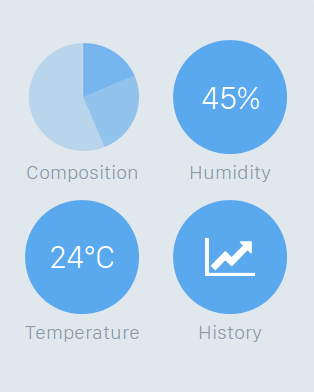
\includegraphics[scale=0.4]{images/home.png}
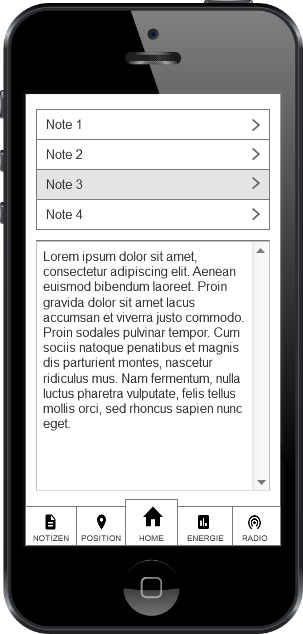
\includegraphics[scale=0.4]{images/notizen.png}
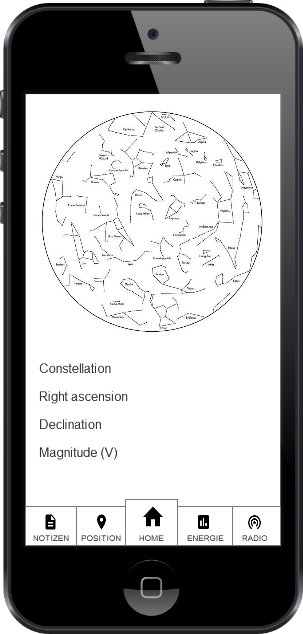
\includegraphics[scale=0.4]{images/position.png}
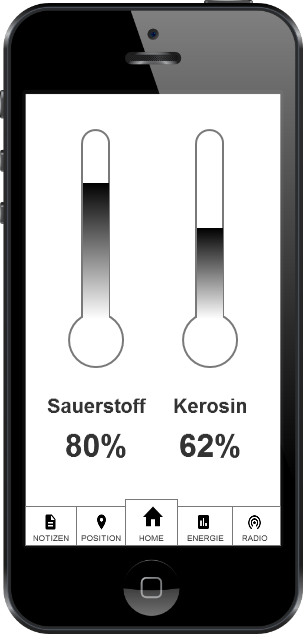
\includegraphics[scale=0.4]{images/energie.png}
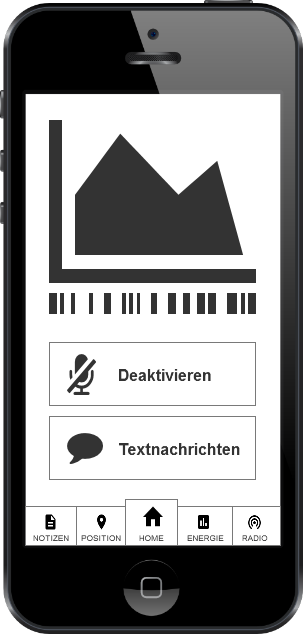
\includegraphics[scale=0.4]{images/radio.png}

\subsection{Home}
Auf dem Start-Screen findet der User eine �bersicht aller Funktionen. 
Die Sprechblasen fungieren f�r neue Nutzern als Erkl�rungshilfe und geben auch sofort einen �berblick �ber alles Wissenswerte.(Instant Gratification) \\
\ \\Um die Bedienung einfacher und eing�niger zu gestalten, haben wir uns in der Start-Zeile f�r Icons und Text entschieden. Der Home-Button ist etwas gr��er um ihn von den anderen abzuheben. �ber diesen kann der Nutzer von jedem anderen Screen zum Start-Screen zur�ckkehren (Safe Exploration/Escape Hatch). \\
\ \\ F�r den Start-Screen benutzen wir die "Home" Metapher, diese ist sehr bekannt und oft verwendet, zusammen mit dem Haus als Icon wird schnell klar was hiermit gemeint ist. 

\subsection{Notizen}
Im oberen Bereich hat der Nutzer eine �bersicht seiner Notizen, und im unteren Bereich die eigentlichen Inhalte, sodass eine klare Teilung entsteht. Der Nutzer muss erst eine Notiz w�hlen, die er angucken m�chte, diese Reihenfolge wird durch die Teilung unterst�zt. \\
\ \\Als Icon haben wir uns f�r einen Notizzettel als offensichtliche Metapher entschieden.

\subsection{Position}
Die Grafik gibt dem Nutzer eine schnelle �bersicht �ber den Sternenhimmel und wo er sich an diesem befindet. Zudem kann er weitere Informationen wie z.B. Neigung oder Aufstieg abrufen. Auch hier wird durch die Visuelle Teilung die Reihenfolge beeinflusst in der der Nutzer die Elemente wahrnimmt, sodass er die wichtigsten Informationen zuerst sieht. \\
\ \\Als Icon benutzen wir den bekannten Orts-Pfeil von z.B. Navigationsger�ten, sodass Nutzer leicht erkennen was dahinter steckt.

\subsection{Energie}
Hier findet der Nutzer eine einfache �bersicht des Sauerstoff und Kerosin-Standes. Zur leichteren Verst�ndlichkeit wird der Stand sowohl als Zahl als auch grafisch dargestellt. \\
\ \\ Das Icon repr�sentiert die tats�chliche Darstellung der Energie-Levels, sodass der Nutzer genau wei�, was ihn erwartet.


\subsection{Radio}
Auf diesem Screen kann der Nutzer mit einem Blick die Verbindungsqualit�t der Spracheinheit einsehen, sein Mikrofon deaktivieren (bzw. wieder aktivieren) oder in einen weiteren Screen f�r Textnachrichten wechseln.
Wie auf den anderen Screens steht auch hier Einfachheit und leichte Bedienung im Vordergrund. 
Der Screen ist zweigeteilt, in den interaktiven Teil unten, und den Informationsteil oben.\\

\ \\ Generell sind alle Screens schlicht gehalten, um nicht vom Inhalt abzulenken, da der Nutzen im Mittelpunkt stehen soll. 

\subsection{Sketches}
\includegraphics[scale=0.4]{images/sketches.JPG}
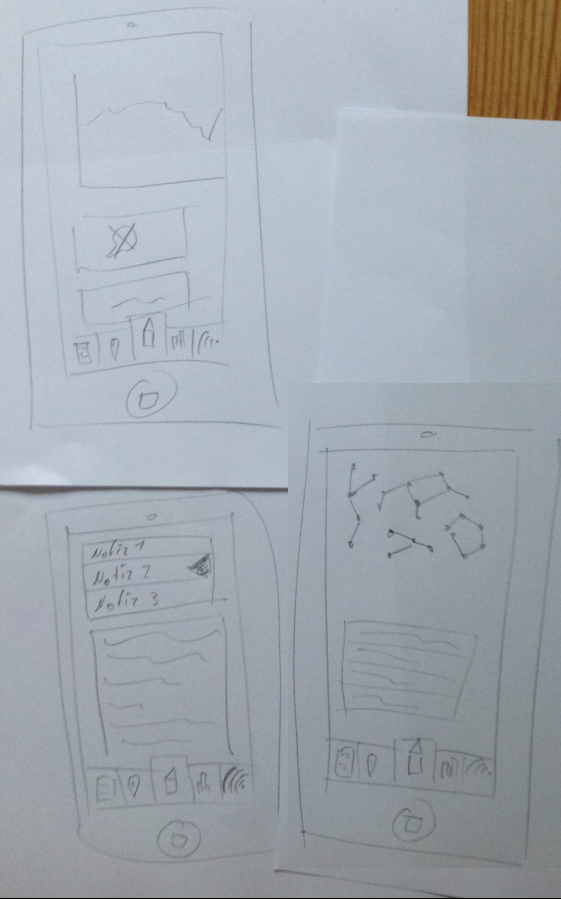
\includegraphics[scale=0.4]{images/sketches2.png}

\end{document}
